%%
%% Beuth Hochschule für Technik --  
%%
%% Kapitel 3 - Desktop App
%%
%%	

\chapter{Desktop App}
Zu der Android App soll es parallel eine App für den Desktop geben. Diese wurde mit mit JavaFX programmiert.
\section{Was ist JavaFX ?}
JavaFX ist eine Java Spezifikation die als Hauptkonkurrenten Adobe Flash und Microsoft Silverlight hat. Ein positiver Punkt ist der Lauffähigkeit auf diversen Geräten wie z.B. Mobilfunk, Desktop-Computern, Embedded Geräten und Blu-ray Geräten. Die Programmierung findet ganz normal wie in Java statt. Die dazu gehörigen Bibliotheken werden seit der Java SE Runtime 7 Update 6 automatisch mit installiert. Es ist unter anderem auf die Grafikprogrammierung ausgelegt. Dadurch lassen sich Grafische Elemente schnell programmieren und mit CSS gestalten.(Quelle: \cite{bib.jFXRaspPi})\newline
Ein sehr bekanntes Embedded Gerät wofür es auch JavaFX gibt ist das Raspberry Pi.
\section{Struktur und Aufbau der App}
Es gibt insgesamt 5 verschiedene Fenster in der App.
\begin{itemize}
	\item Login (siehe \ref{subsec.login})
	\item Registrierung (siehe \ref{subsec.registrierung})
	\item Control (siehe \ref{subsec.control})
	\item Datenbank (siehe \ref{subsec.datenbank})
	\item Foto (siehe \ref{subsec.foto})
\end{itemize}

\begin{figure}[H]
  \begin{center}
    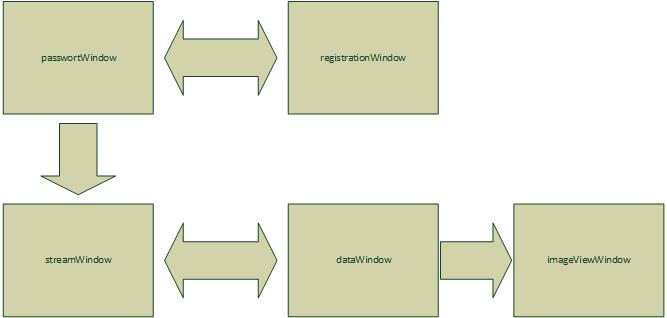
\includegraphics[width=\linewidth]{MaskenDesktopVersion.jpg}
  		  \caption{Namen der View müssen noch geändert werden}
  		%  \footnotesize{Quelle: \cite{RolfKlaus}}
     \label{fig.C167}
  \end{center}
\end{figure}

\subsection{Login}
\label{subsec.login}
Bei dem Login Fenster muss sich der Nutzer mit seinem Usernamen und Passwort was in der Datenbank hinterlegt ist anmelden. Es ist ihm die Möglichkeit gegeben sein Passwort sich in Klartext anzuzeigen zu lassen. Wird der OK - Button betätigt wird eine Verbindung zur Datenbank hergestellt und die eingegebenen Daten auf Korrektheit überprüft. Hat der Benutzer noch kein Konto in der Datenbank kann er sich über den Registrierung - Button registrieren.

\subsection{Registrierung}
\label{subsec.registrierung}

\subsection{Control}
\label{subsec.control}

\subsection{Datenbank}
\label{subsec.datenbank}

\subsection{Foto}
\label{subsec.foto}